%%%%%%%%%%%%%%%%%%%%%%%%%%%%%%%%%%%%%%%%%
% Tech United Beamer Presentation
% LaTeX Template
% Version 1.0 (10/11/12)
% License:
% CC BY-NC-SA 3.0 (http://creativecommons.org/licenses/by-nc-sa/3.0/)
%%%%%%%%%%%%%%%%%%%%%%%%%%%%%%%%%%%%%%%%%%

\documentclass[aspectratio=43]{beamer}

\mode<presentation> {
	\setbeamertemplate{navigation symbols}{} % To remove the navigation symbols from the bottom of all slides uncomment this line
}

\usepackage{epstopdf}
\usepackage{color}
\usepackage{graphicx} % Allows including images
\usepackage{hyperref}
\usepackage{subfigure}
\usepackage{multicol}
\usepackage{nameref}  % Package which allows us to read the current label
\usepackage{caption}
\usepackage{array}
\usepackage{enumitem,xcolor} % TechUnitedItemize
\usepackage{tikz}
\usepackage{booktabs}
\usepackage[absolute,overlay]{textpos}
\usepackage{media9}
\usepackage{etoolbox}

%% COLOR DEFINITIONS
\definecolor{TechUnitedOrange}{rgb}{0.98, 0.659, 0.212}
\definecolor{TechUnitedGreen}{rgb}{0.034, 0.619, 0.352}
\newcommand{\Techemph}[1]{\textcolor{TechUnitedGreen}{#1}}
\newcommand{\coloremph}[1]{\textcolor{blue}{#1}}

%% TECH UNITED ITEMIZE
\setbeamertemplate{itemize items}[circle]
\newlist{TechUnitedItems}{itemize}{1}
\setlist[TechUnitedItems]{label=\textcolor{TechUnitedGreen}{\textbullet}}

%% TECH UNITED SHIELD
\newcommand{\TechUnitedShield}[1]{
	\iftoggle{#1}{ % 16_9

	}{ % 4_3
	\begin{textblock*}{2.6cm}(100mm,-3mm)
			\begin{figure}
				\centering
				
\includegraphics[width=2.6cm]{../[TechUnitedStyle]/Figures/Logo's/TechUnitedTransparant_burned.png}
			\end{figure}
	\end{textblock*}
	}
}

\newcommand{\TechUnitedTitle}[1]{
	\begin{textblock*}{\paperwidth}(10mm,4mm)
		{\huge\textcolor{TechUnitedOrange}{#1}}
	\end{textblock*}
}
\newcommand{\TechUnitedPicture}[2]{
	\begin{textblock*}{\paperwidth}(-15mm,12.5mm)
		\begin{figure}
			\centering
			\includegraphics[width=0.65\linewidth,trim={0 20mm 0 80mm},clip]{#1}
		\end{figure}
	\end{textblock*}
	\TechUnitedPictureText{#2}
}

\newcommand{\TechUnitedPictureNoText}[1]{
	\begin{textblock*}{\paperwidth}(-15mm,12.5mm)
		\begin{figure}
			\centering
			\includegraphics[width=0.65\linewidth,trim={0 15mm 0 15mm},clip]{#1}
		\end{figure}
	\end{textblock*}
}

\newcommand{\TechUnitedPictureText}[1]{
	\begin{textblock*}{35mm}(120mm,48mm)
		\begin{center}
			{\large "\textit{#1}"}
		\end{center}
	\end{textblock*}
}

\newcommand{\TechUnitedYoutube}[2]{
	\iftoggle{#1}{ % 16_9
		
	}{ % 4_3
		\begin{textblock*}{128mm}(0pt,13.2mm)
			\includemedia[
			width=128mm,height=75.1mm,
			activate=pageopen,
			flashvars={
				modestbranding=1 % no YT logo in control bar
				&autohide=1       % controlbar autohide
				&showinfo=0       % no title and other info before start
			}
			]{}{#2}
		\end{textblock*}
	}
}

\newcommand{\TechUnitedMovie}[2]{
	\iftoggle{#1}{ % 16_9
		
	}{ % 4_3
		\begin{textblock*}{\paperwidth}(0pt,13.2mm)
			\includemedia[
			width=128mm,
			height=75.1mm, % This used to be 75.1mm
			activate=pageopen,
			addresource=#2,
			flashvars={source=#2}
			]{}{VPlayer9.swf}

%\includemedia[
%  activate=pageopen,
%  width=240pt,height=150pt,
%  addresource=#2,
%  flashvars={%
%src=#2      % same path as in addresource!
%%&scaleMode=stretch % removes black bars
%&autoPlay=true      % optional configuration
%&loop=true          % variables
%}
%]{}{StrobeMediaPlayback.swf}
		\end{textblock*}
	}
}

\newcommand{\TechUnitedTitleBackground}[1]{
	\usebackgroundtemplate{
		\iftoggle{#1}{
			
\includegraphics[width=\paperwidth,height=\paperheight]{../[TechUnitedStyle]/Backgrounds/TitlePageTechUnited_16_9.eps}%
		}{
			
\includegraphics[width=\paperwidth,height=\paperheight]{../[TechUnitedStyle]/Backgrounds/TitlePageTechUnited_4_3.eps}%
		}
	}
}

\newcommand{\TechUnitedTitlePage}[3]{
	\begin{frame}
		\iftoggle{#3}{
	
		}{
			\begin{textblock*}{120mm}(0mm,12mm)
				\begin{flushright}
					\LARGE\textcolor{white}{\textbf{#1}}
				\end{flushright}
			\end{textblock*}
			\begin{textblock*}{120mm}(0mm,24mm)
				\begin{flushright}
					\textcolor{white}{\textbf{By: #2}}
				\end{flushright}
			\end{textblock*}
			\begin{textblock*}{3.0cm}(10mm,42mm)
				\begin{figure}
					\centering
					
\includegraphics[width=3.0cm]{../[TechUnitedStyle]/Figures/Logo's/TechUnitedTransparant_burned.png}
				\end{figure}
			\end{textblock*}
			\begin{textblock*}{3.0cm}(10mm,78mm)
				\begin{figure}
					\centering
					
\includegraphics[width=3.0cm]{../[TechUnitedStyle]/Figures/Logo's/TUETransparent.png}
				\end{figure}
			\end{textblock*}
			\begin{textblock*}{5mm}(50mm,53.5mm)
				
\includegraphics[width=\linewidth]{../[TechUnitedStyle]/Figures/TitlePageLogo's/Facebook.png}
			\end{textblock*}
			\begin{textblock*}{5mm}(50mm,61mm)
				
\includegraphics[width=\linewidth]{../[TechUnitedStyle]/Figures/TitlePageLogo's/Twitter.png}
			\end{textblock*}
			\begin{textblock*}{5mm}(50mm,67mm)
				
\includegraphics[width=\linewidth]{../[TechUnitedStyle]/Figures/TitlePageLogo's/Email.png}
			\end{textblock*}
			\begin{textblock*}{5mm}(50mm,74mm)
				
\includegraphics[width=\linewidth]{../[TechUnitedStyle]/Figures/TitlePageLogo's/Internet.png}
			\end{textblock*}
			\begin{textblock*}{50mm}(58mm,55mm)
				\textcolor{white}{
					Tech United Eindhoven \vspace{0.5em}\\
					@TechUnited \vspace{0.5em}\\
					techunited@tue.nl \vspace{0.5em}\\
					www.techunited.nl
				}
			\end{textblock*}
		}
	\end{frame}
}

\newcommand{\TechUnitedFinalSlide}[1]{
	\iftoggle{#1}{
	}{
		\begin{frame}
			\begin{textblock*}{\paperwidth}(0mm,18mm)
				{\begin{center}
						\LARGE\textcolor{white}{\textbf{Thank you for your attention!}}
					\end{center}
				}
			\end{textblock*}
			\begin{textblock*}{3.0cm}(10mm,42mm)
				\begin{figure}
					\centering
					
\includegraphics[width=3.0cm]{../[TechUnitedStyle]/Figures/Logo's/TechUnitedTransparant_burned.png}
				\end{figure}
			\end{textblock*}
			\begin{textblock*}{3.0cm}(10mm,78mm)
				\begin{figure}
					\centering
					
\includegraphics[width=3.0cm]{../[TechUnitedStyle]/Figures/Logo's/TUETransparent.png}
				\end{figure}
			\end{textblock*}
			\begin{textblock*}{5mm}(50mm,53.5mm)
				
\includegraphics[width=\linewidth]{../[TechUnitedStyle]/Figures/TitlePageLogo's/Facebook.png}
			\end{textblock*}
			\begin{textblock*}{5mm}(50mm,61mm)
				
\includegraphics[width=\linewidth]{../[TechUnitedStyle]/Figures/TitlePageLogo's/Twitter.png}
			\end{textblock*}
			\begin{textblock*}{5mm}(50mm,67mm)
				
\includegraphics[width=\linewidth]{../[TechUnitedStyle]/Figures/TitlePageLogo's/Email.png}
			\end{textblock*}
			\begin{textblock*}{5mm}(50mm,74mm)
				
\includegraphics[width=\linewidth]{../[TechUnitedStyle]/Figures/TitlePageLogo's/Internet.png}
			\end{textblock*}
			\begin{textblock*}{50mm}(58mm,55mm)
				\textcolor{white}{
					Tech United Eindhoven \vspace{0.5em}\\
					@TechUnited \vspace{0.5em}\\
					techunited@tue.nl \vspace{0.5em}\\
					www.techunited.nl
				}
			\end{textblock*}
		\end{frame}
	}
}

\newcommand{\TechUnitedSheetBackground}[1]{
	\usebackgroundtemplate{
		\iftoggle{#1}{
			
\includegraphics[width=\paperwidth,height=\paperheight]{../[TechUnitedStyle]/Backgrounds/TotalOverlay_16_9.eps}%
		}{
			
\includegraphics[width=\paperwidth,height=\paperheight]{../[TechUnitedStyle]/Backgrounds/TotalOverlay_4_3.eps}%
		}
	}
}





\newcolumntype{C}[1]{>{\centering\let\newline\\\arraybackslash\hspace{0pt}}m{#1}}
\newcolumntype{R}[1]{>{
		\begin{flushright}
			\let\newline\\\arraybackslash\hspace{0pt}
	\end{flushright}}m{#1}
}

%% CONFERENCE OR WEB VERSION! %%
\newtoggle{ConferenceNotWeb}
%\toggletrue{ConferenceNotWeb}
\togglefalse{ConferenceNotWeb}
%% CONFERENCE OR WEB VERSION! %%

%% 16/9 OR 4/3! %%
\newtoggle{16_9_not_4_3}
%% 16/9 OR 4/3! %%

\newcommand*{\currentname}{\@currentlabelname}
\makeatletter 

\togglefalse{16_9_not_4_3}
%----------------------------------------------------------------------------------------
%	TITLE PAGE
%----------------------------------------------------------------------------------------

\newcommand{\TULeftMargin}{0.05\paperwidth}
\newcommand{\TULeftWidth}{0.4\paperwidth}
\newcommand{\TURightMargin}{0.50\paperwidth}
\newcommand{\TURightWidth}{0.45\paperwidth}

\begin{document}
	\TechUnitedTitleBackground{16_9_not_4_3}
	\TechUnitedTitlePage{Presentation @Home team}{Amigo \& the demo team}{16_9_not_4_3}
	% -------------------------------------------------------------
	% 					Start of Content
	% -------------------------------------------------------------
	\TechUnitedSheetBackground{16_9_not_4_3}
	
%%Slide 2
	\begin{frame}\TechUnitedTitle{Robotics team of the TU/e}\TechUnitedShield{16_9_not_4_3}
	
		\begin{textblock*}{\TULeftWidth}(\TULeftMargin,20mm)
			\begin{figure}
				\centering
				\includegraphics[width=0.7\linewidth]{[TechUnitedStyle]/Figures/Turtle}
			\end{figure}
		\end{textblock*}
		
		\begin{textblock*}{\TURightWidth}(\TURightMargin,50mm)
			\textbf{Middle Size League (MSL)}
	\end{textblock*}
	
	\end{frame}



%%Slide 3
	\begin{frame}\TechUnitedTitle{Robotics team of the TU/e}\TechUnitedShield{16_9_not_4_3}
	
		\begin{textblock*}{\TULeftWidth}(\TULeftMargin,15mm)
			\begin{figure}
				\centering
				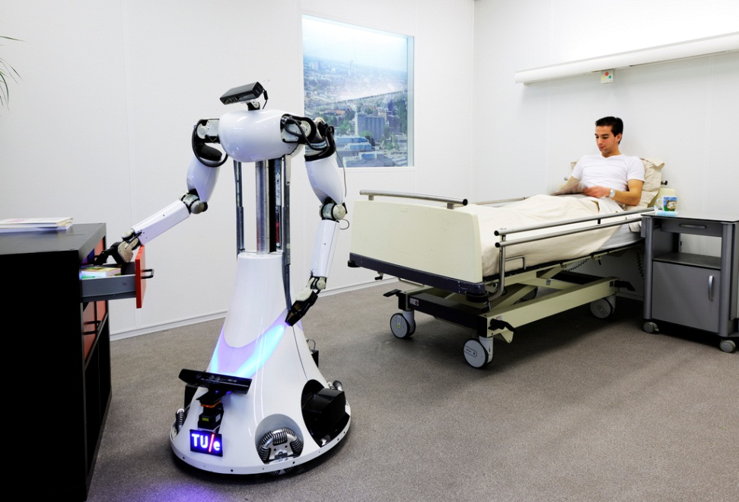
\includegraphics[width=1.9\linewidth]{[TechUnitedStyle]/Figures/AtHome}
			\end{figure}
		\end{textblock*}
		
		\begin{textblock*}{\TURightWidth}(\TURightMargin,80mm)
			\Large\textbf{ @Home team}
	\end{textblock*}
	
	\end{frame}

%%Slide 4
	\begin{frame}\TechUnitedTitle{Robotics team of the TU/e}\TechUnitedShield{16_9_not_4_3}
	
		\begin{textblock*}{\TULeftWidth}(\TULeftMargin,15	mm)
			\begin{figure}
				\centering
				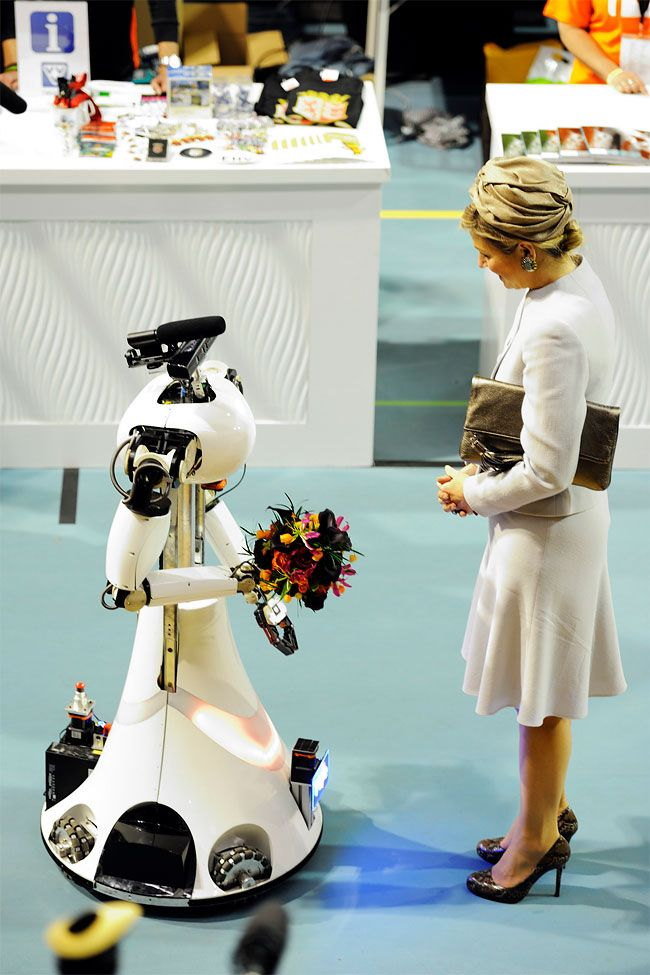
\includegraphics[width=0.8\linewidth]{[TechUnitedStyle]/Figures/Maxima}
			\end{figure}
		\end{textblock*}
		
		\begin{textblock*}{\TURightWidth}(\TURightMargin,35mm)
			Meet AMIGO! 
			\begin{TechUnitedItems}
				\item Autonomous Mate for IntelliGent Operations
				\item Human like
				\item Height: 1.5 meter
				\item Weight: 80 kg
				\item 15 - 30 minutes battery power
			
			\end{TechUnitedItems}
			
	\end{textblock*}
	
	\end{frame}


%%Slide 5	
\begin{frame}\TechUnitedTitle{Challenges}
		\TechUnitedYoutube{16_9_not_4_3}{https://www.youtube.com/v/p3I3dWwXwi4}
	\end{frame}	
	
%http://www.youtube.com/v/vT-21cQa2_c?rel=0&start=0&version=3
%



%%Slide 6
	\begin{frame}\TechUnitedTitle{Omni-wheels}\TechUnitedShield{16_9_not_4_3}
	
		\begin{textblock*}{\TULeftWidth}(\TULeftMargin,30mm)
			\begin{figure}
				\centering
				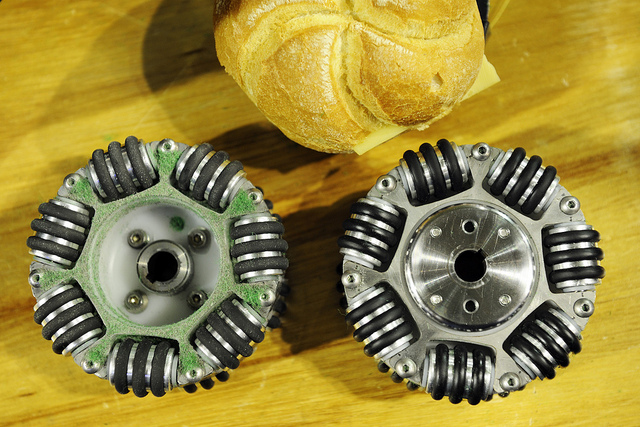
\includegraphics[width=1.1\linewidth]{[TechUnitedStyle]/Figures/Omniwielen}
			\end{figure}
		\end{textblock*}
		
		\begin{textblock*}{\TURightWidth}(\TURightMargin,35mm)
			 Drive anywhere needed or wanted!
			\begin{TechUnitedItems}
				\item 4 implemented wheels
				\item Driven in 1 direction
				\item Friction-free in other directions
				\item Rubber rollers	
			
			\end{TechUnitedItems}
			
	\end{textblock*}
	
	\end{frame}
	
	
	%%Slide 7
	\begin{frame}\TechUnitedTitle{'Seeing' the world}\TechUnitedShield{16_9_not_4_3}
	
		\begin{textblock*}{\TULeftWidth}(\TULeftMargin,20mm)
			\begin{figure}
				\centering
				\includegraphics[width=1\linewidth]{[TechUnitedStyle]/Figures/Kinect}
			\end{figure}
		\end{textblock*}
		
	\begin{textblock*}{\TURightWidth}(\TURightMargin,25mm)
		
			\begin{itemize}
				\item[\textcolor{TechUnitedGreen}{\textbf{I}}] 2 lasers
				\begin{TechUnitedItems}
						\item Collision avoidance
						\item Torso \& base	
				\end{TechUnitedItems}
				\item[\textcolor{TechUnitedGreen}{\textbf{II.}}] Kinect V2
				\begin{TechUnitedItems}
						\item Xbox
						\item Differentiate objects
						\item Recognizing people  
				\end{TechUnitedItems}
				\item[\textcolor{TechUnitedGreen}{\textbf{III.}}] World model
				\begin{TechUnitedItems}
						\item Software based
						\item Mostly human made
						\item Amigo makes small adjustments
				\end{TechUnitedItems}
			\end{itemize}
	\end{textblock*}	
		
\end{frame}

%%Slide 8
	\begin{frame}\TechUnitedTitle{Arms \& Torso}\TechUnitedShield{16_9_not_4_3}
	
		\begin{textblock*}{\TULeftWidth}(\TULeftMargin,15mm)
			\begin{figure}
				\centering
				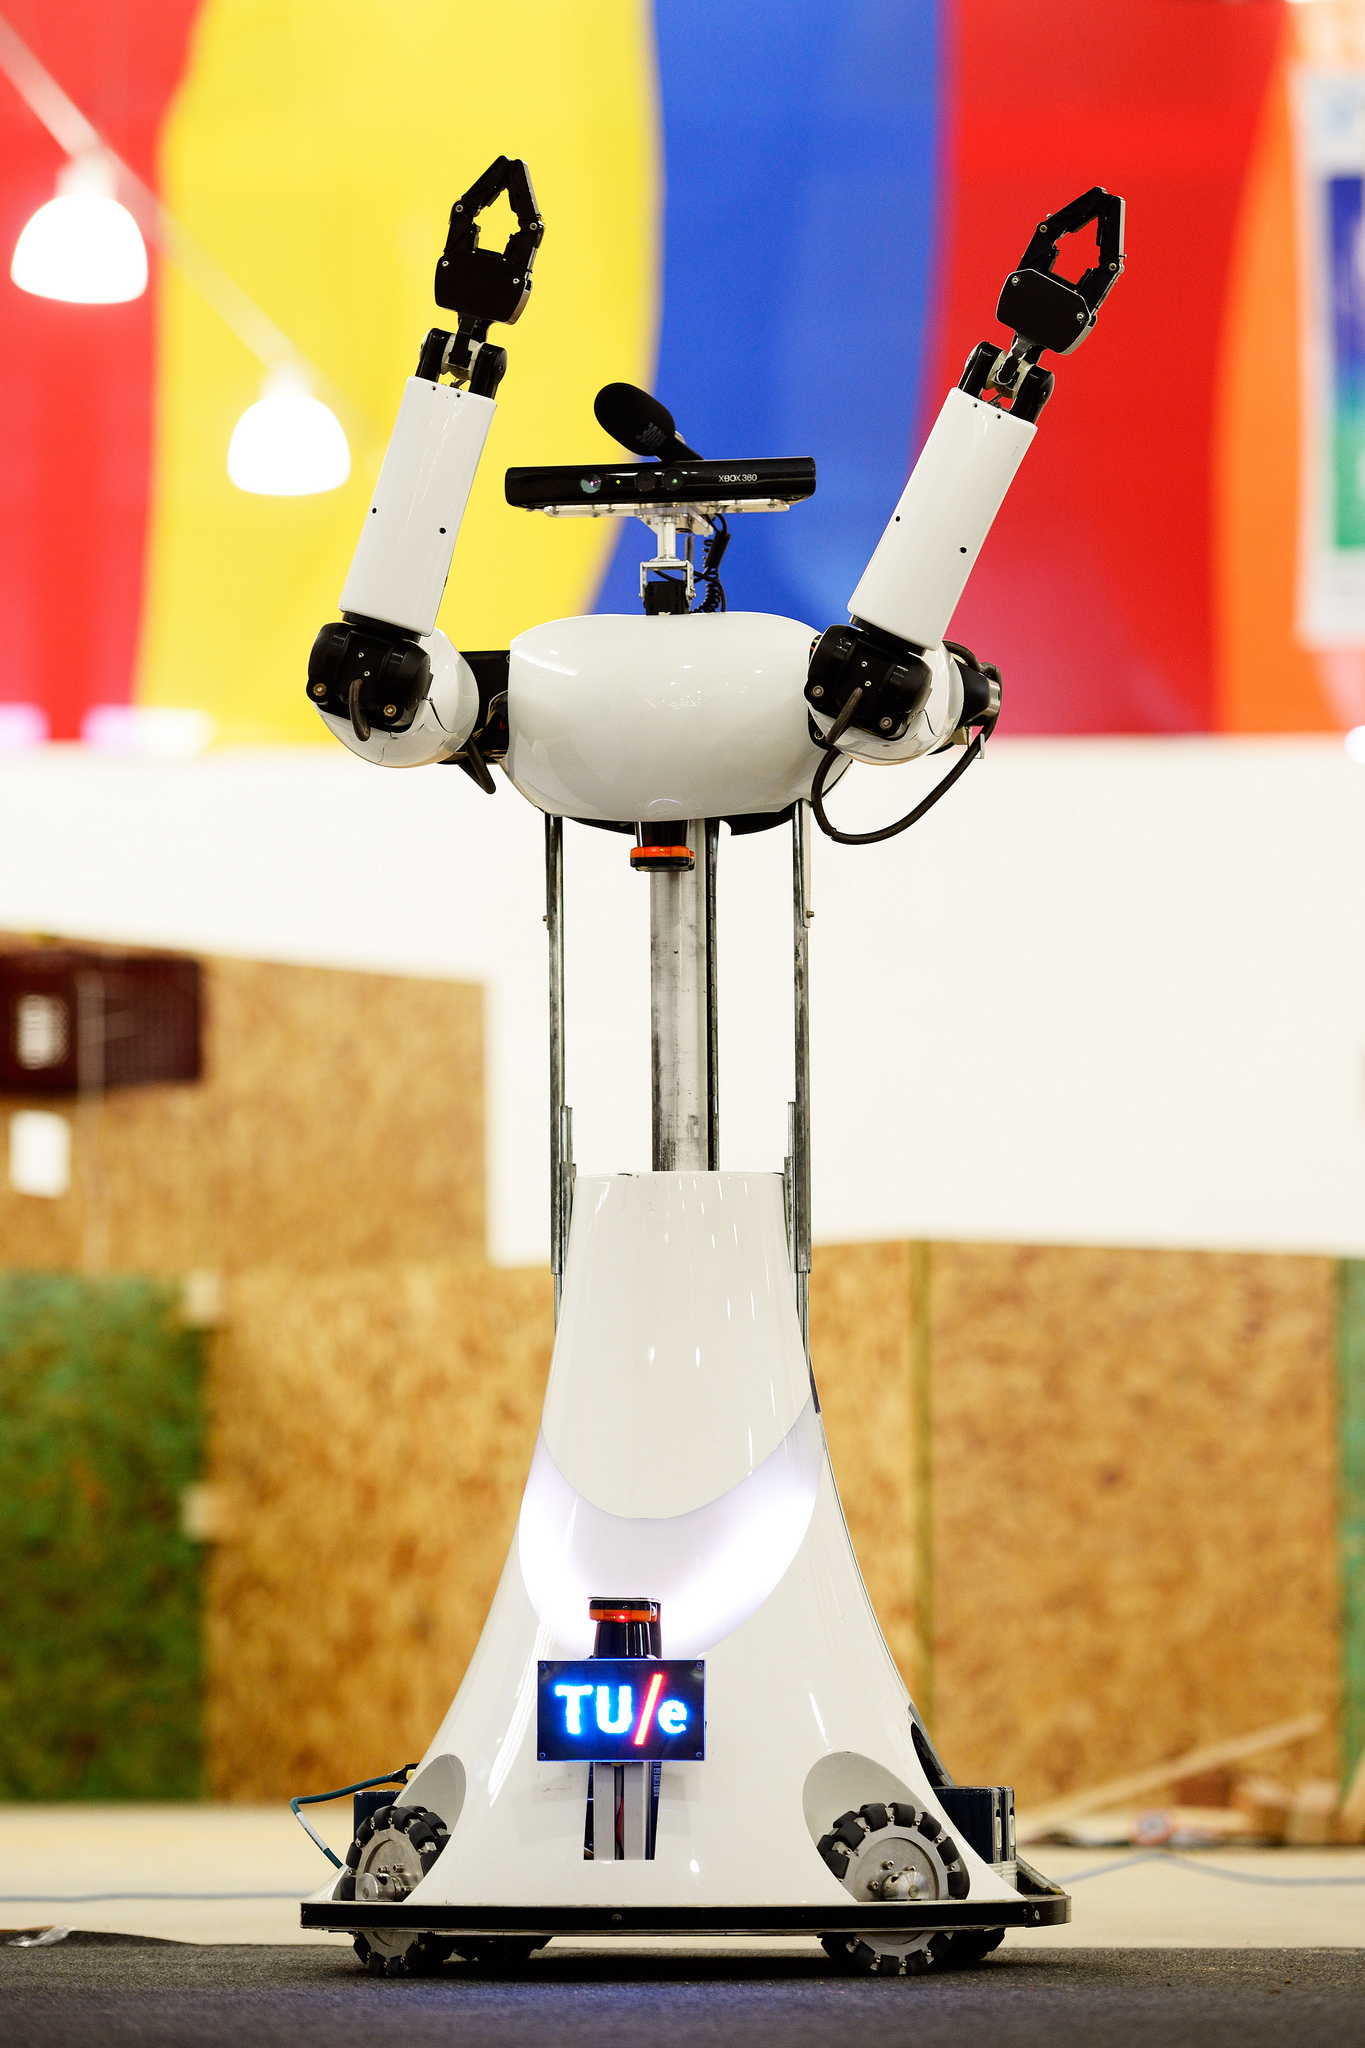
\includegraphics[width=0.8\linewidth]{[TechUnitedStyle]/Figures/Arms}
			\end{figure}
		\end{textblock*}
		
	\begin{textblock*}{\TURightWidth}(\TURightMargin,35mm)
		
			\begin{itemize}
				\item[\textcolor{TechUnitedGreen}{\textbf{I}}] Torso
				\begin{TechUnitedItems}
						\item Moveable up and down
						\item Reach different heights	
				\end{TechUnitedItems}
				
				\item[\textcolor{TechUnitedGreen}{\textbf{II.}}] Arms
				\begin{TechUnitedItems}
						\item Human like 
						\item 1 hand position $\rightarrow$ different arm positions
						  
				\end{TechUnitedItems}
			\end{itemize}
	\end{textblock*}	
	
	\end{frame}

	% -------------------------------------------------------------
	% 					End of Content
	% -------------------------------------------------------------
%	
	
	
	\TechUnitedTitleBackground{16_9_not_4_3}
	\TechUnitedFinalSlide{16_9_not_4_3}

\end{document} 